% Chapter Template

\chapter{实验成果} % Main chapter title

\label{Chapter5} % Change X to a consecutive number; for referencing this chapter elsewhere, use \ref{ChapterX}
我们最终的成果分为三个版本,其中包括基础功能的CPU,与键盘VGA交互的CPU,同时运行两套监控程序的CPU。下面将列举实验的一些成果。

%----------------------------------------------------------------------------------------
%	SECTION 1
%----------------------------------------------------------------------------------------

\section{基础版本CPU}

我们CPU使用的时钟为25M,可以正确执行30条指令,并对冲突有很好地处理。根据测试样例程序的的指令总数和运行时间,可以看出我们的CPU主频确实达到了25M。

\begin{figure}[H]
  \centering
  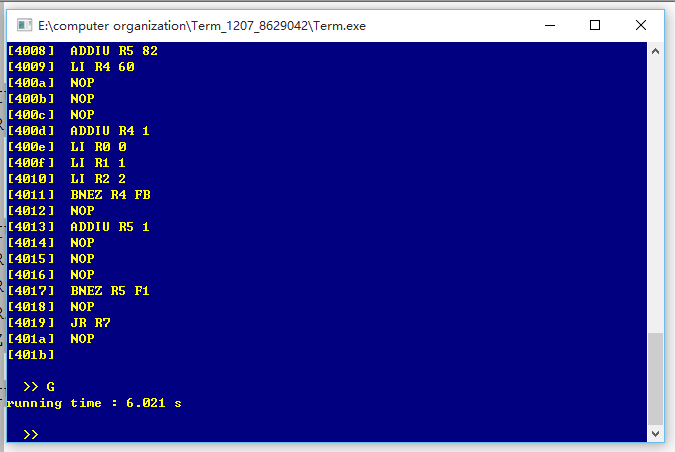
\includegraphics[width=5in]{Figures/cpu1.png}
  \caption{测试程序1}
\end{figure}

\begin{figure}[H]
  \centering
  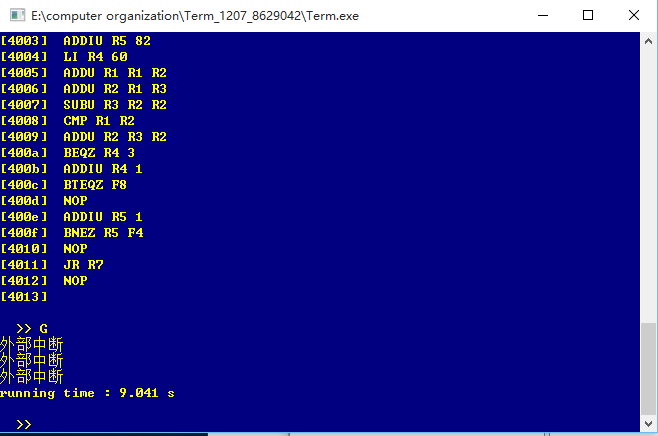
\includegraphics[width=5in]{Figures/cpu2.png}
  \caption{测试程序2}
\end{figure}

\begin{figure}[H]
  \centering
  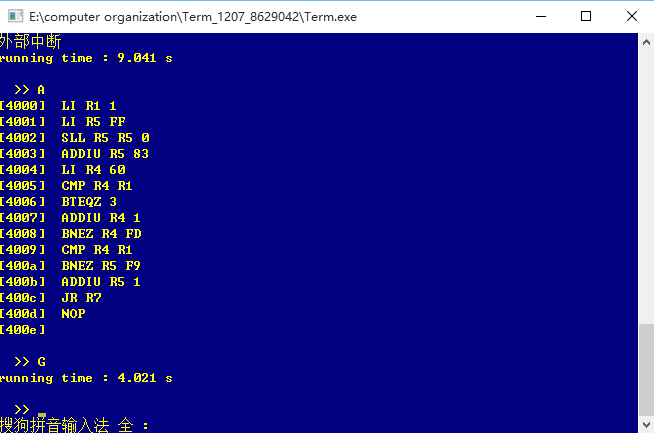
\includegraphics[width=5in]{Figures/cpu3.png}
  \caption{测试程序3}
\end{figure}

\begin{figure}[H]
  \centering
  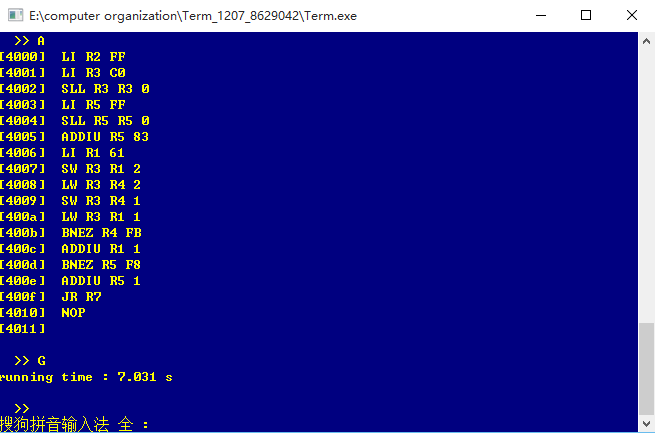
\includegraphics[width=5in]{Figures/cpu4.png}
  \caption{测试程序4}
\end{figure}

\begin{figure}[H]
  \centering
  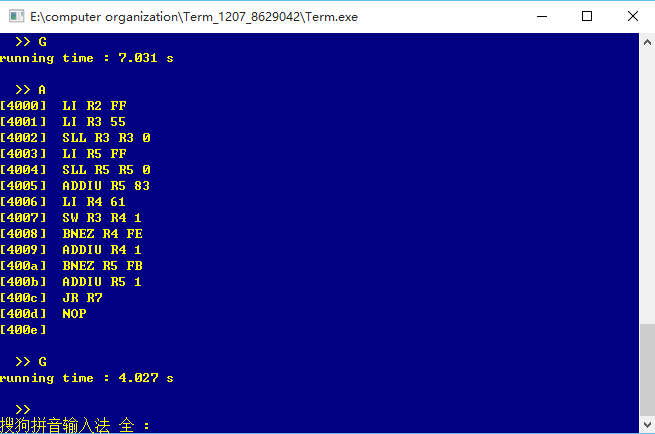
\includegraphics[width=5in]{Figures/cpu5.png}
  \caption{测试程序5}
\end{figure}

在测试程序2中,我们在运行期间通过手动clk产生中断信号,可以看到term中出现了“硬件中断”字样。

%----------------------------------------------------------------------------------------
%	SECTION 2
%----------------------------------------------------------------------------------------

\section{键盘VGA版本CPU}

键盘VGA版本的CPU并没有改变CPU内核代码,所以时钟仍为25M。以下为我们拍摄的一些实验结果。

运行程序,可以看到VGA上显示出OK字样。并通过R指令查用户寄存器的值。后面我们通过键盘输入组合键,可以看到VGA可以正确地显示出字符。

\begin{figure}[H]
  \centering
  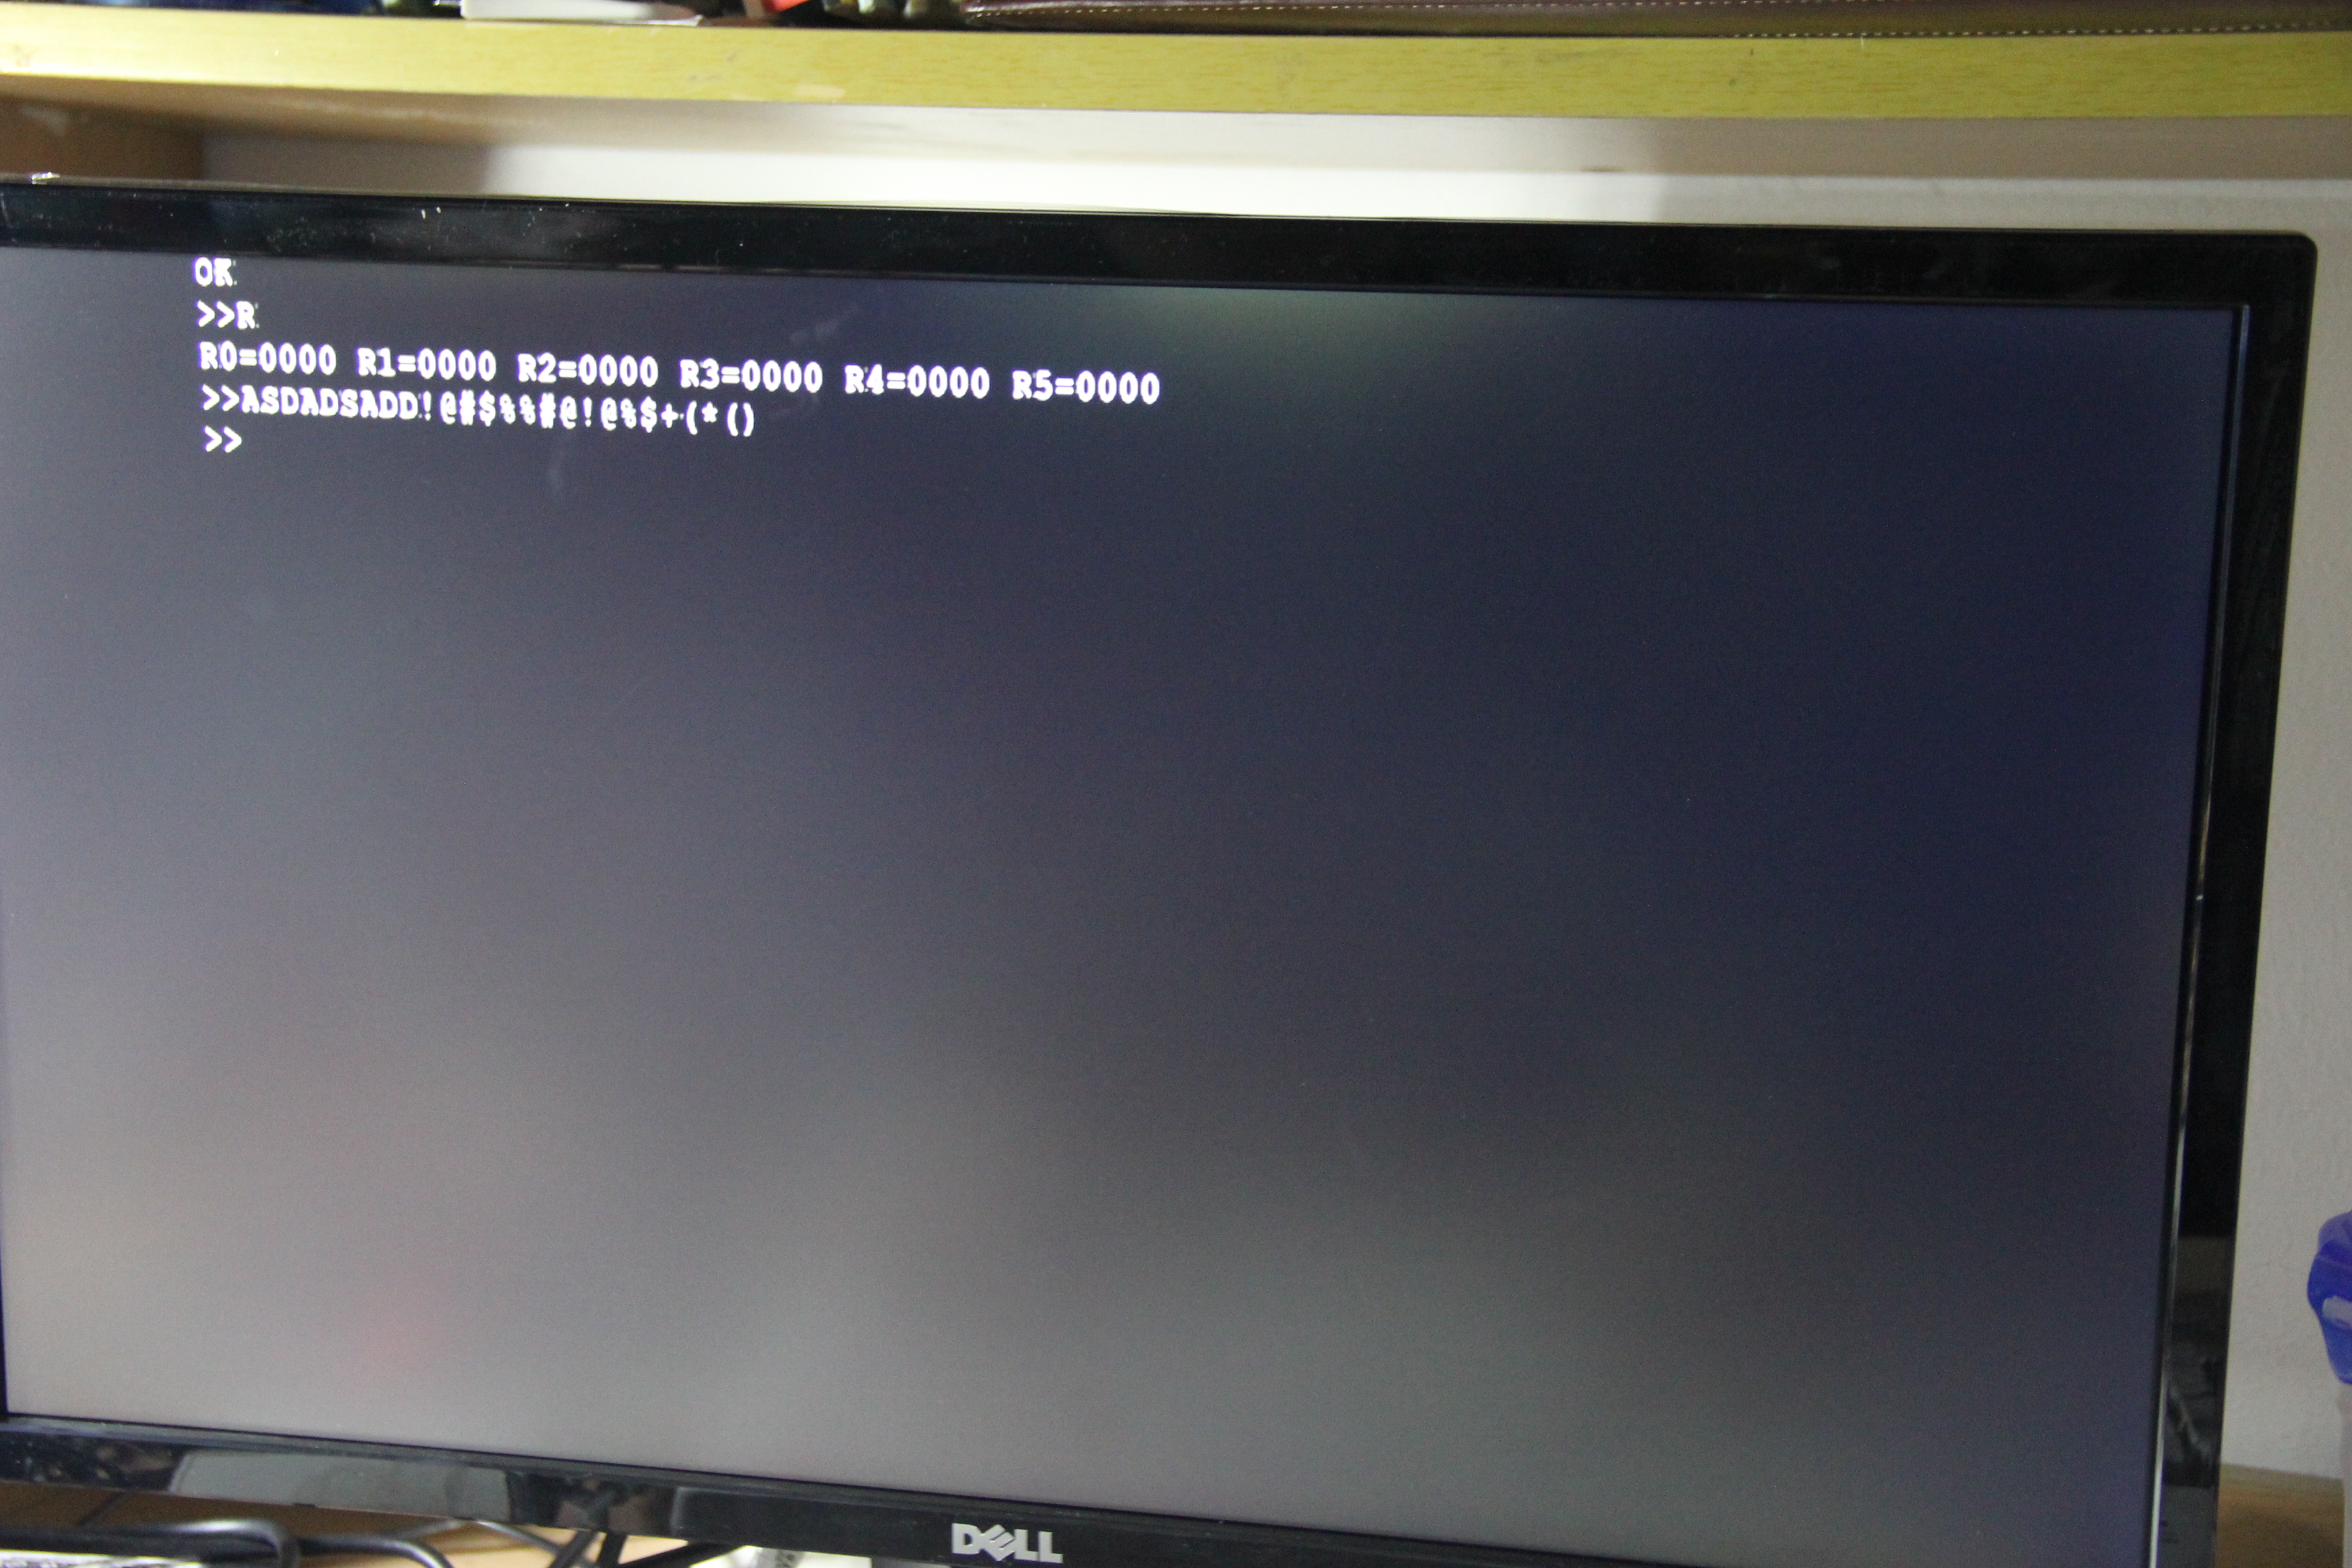
\includegraphics[width=4.5in]{Figures/picture/IMG_7232.JPG}
  \caption{R指令}
\end{figure}

我们在几秒钟没有操作之后,进入屏幕保护界面。

\begin{figure}[H]
  \centering
  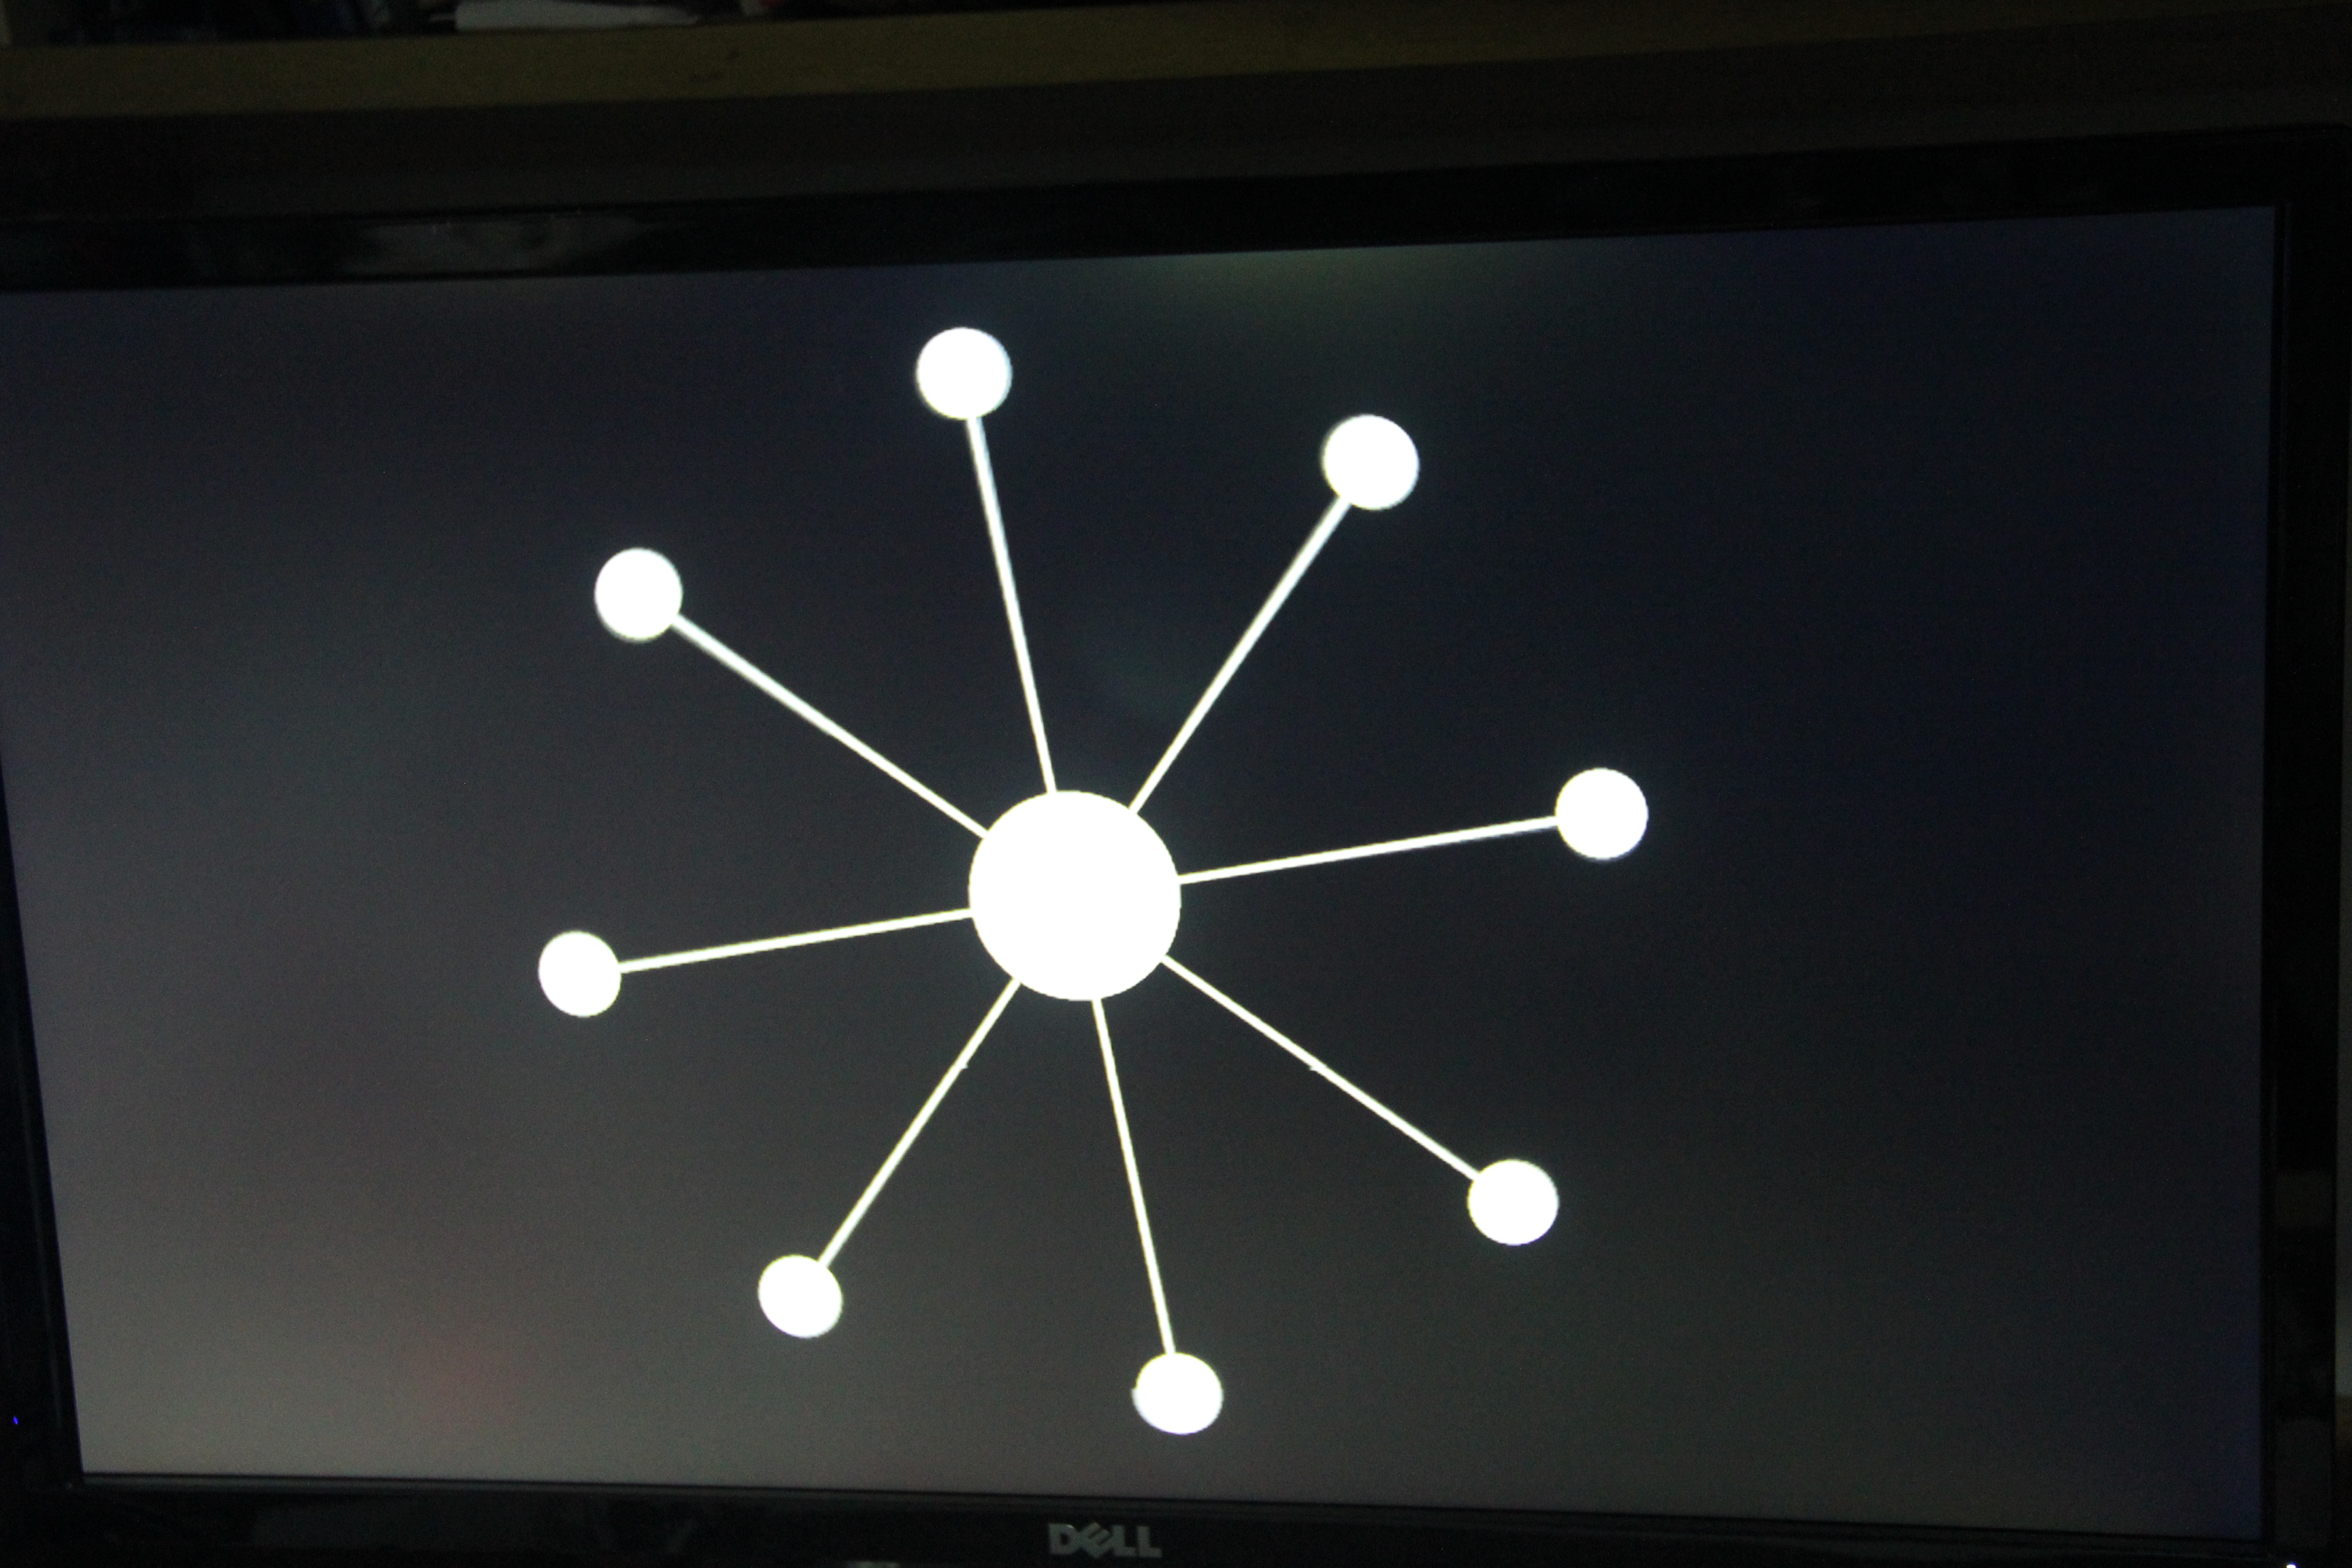
\includegraphics[width=4.5in]{Figures/picture/IMG_7233.JPG}
  \caption{屏幕保护}
\end{figure}

我们通过A指令写入汇编代码,A指令同时支持增加写入地址的参数。同时,我们通过U指令反汇编出刚写入的指令,检查正确性。

\begin{figure}[H]
  \centering
  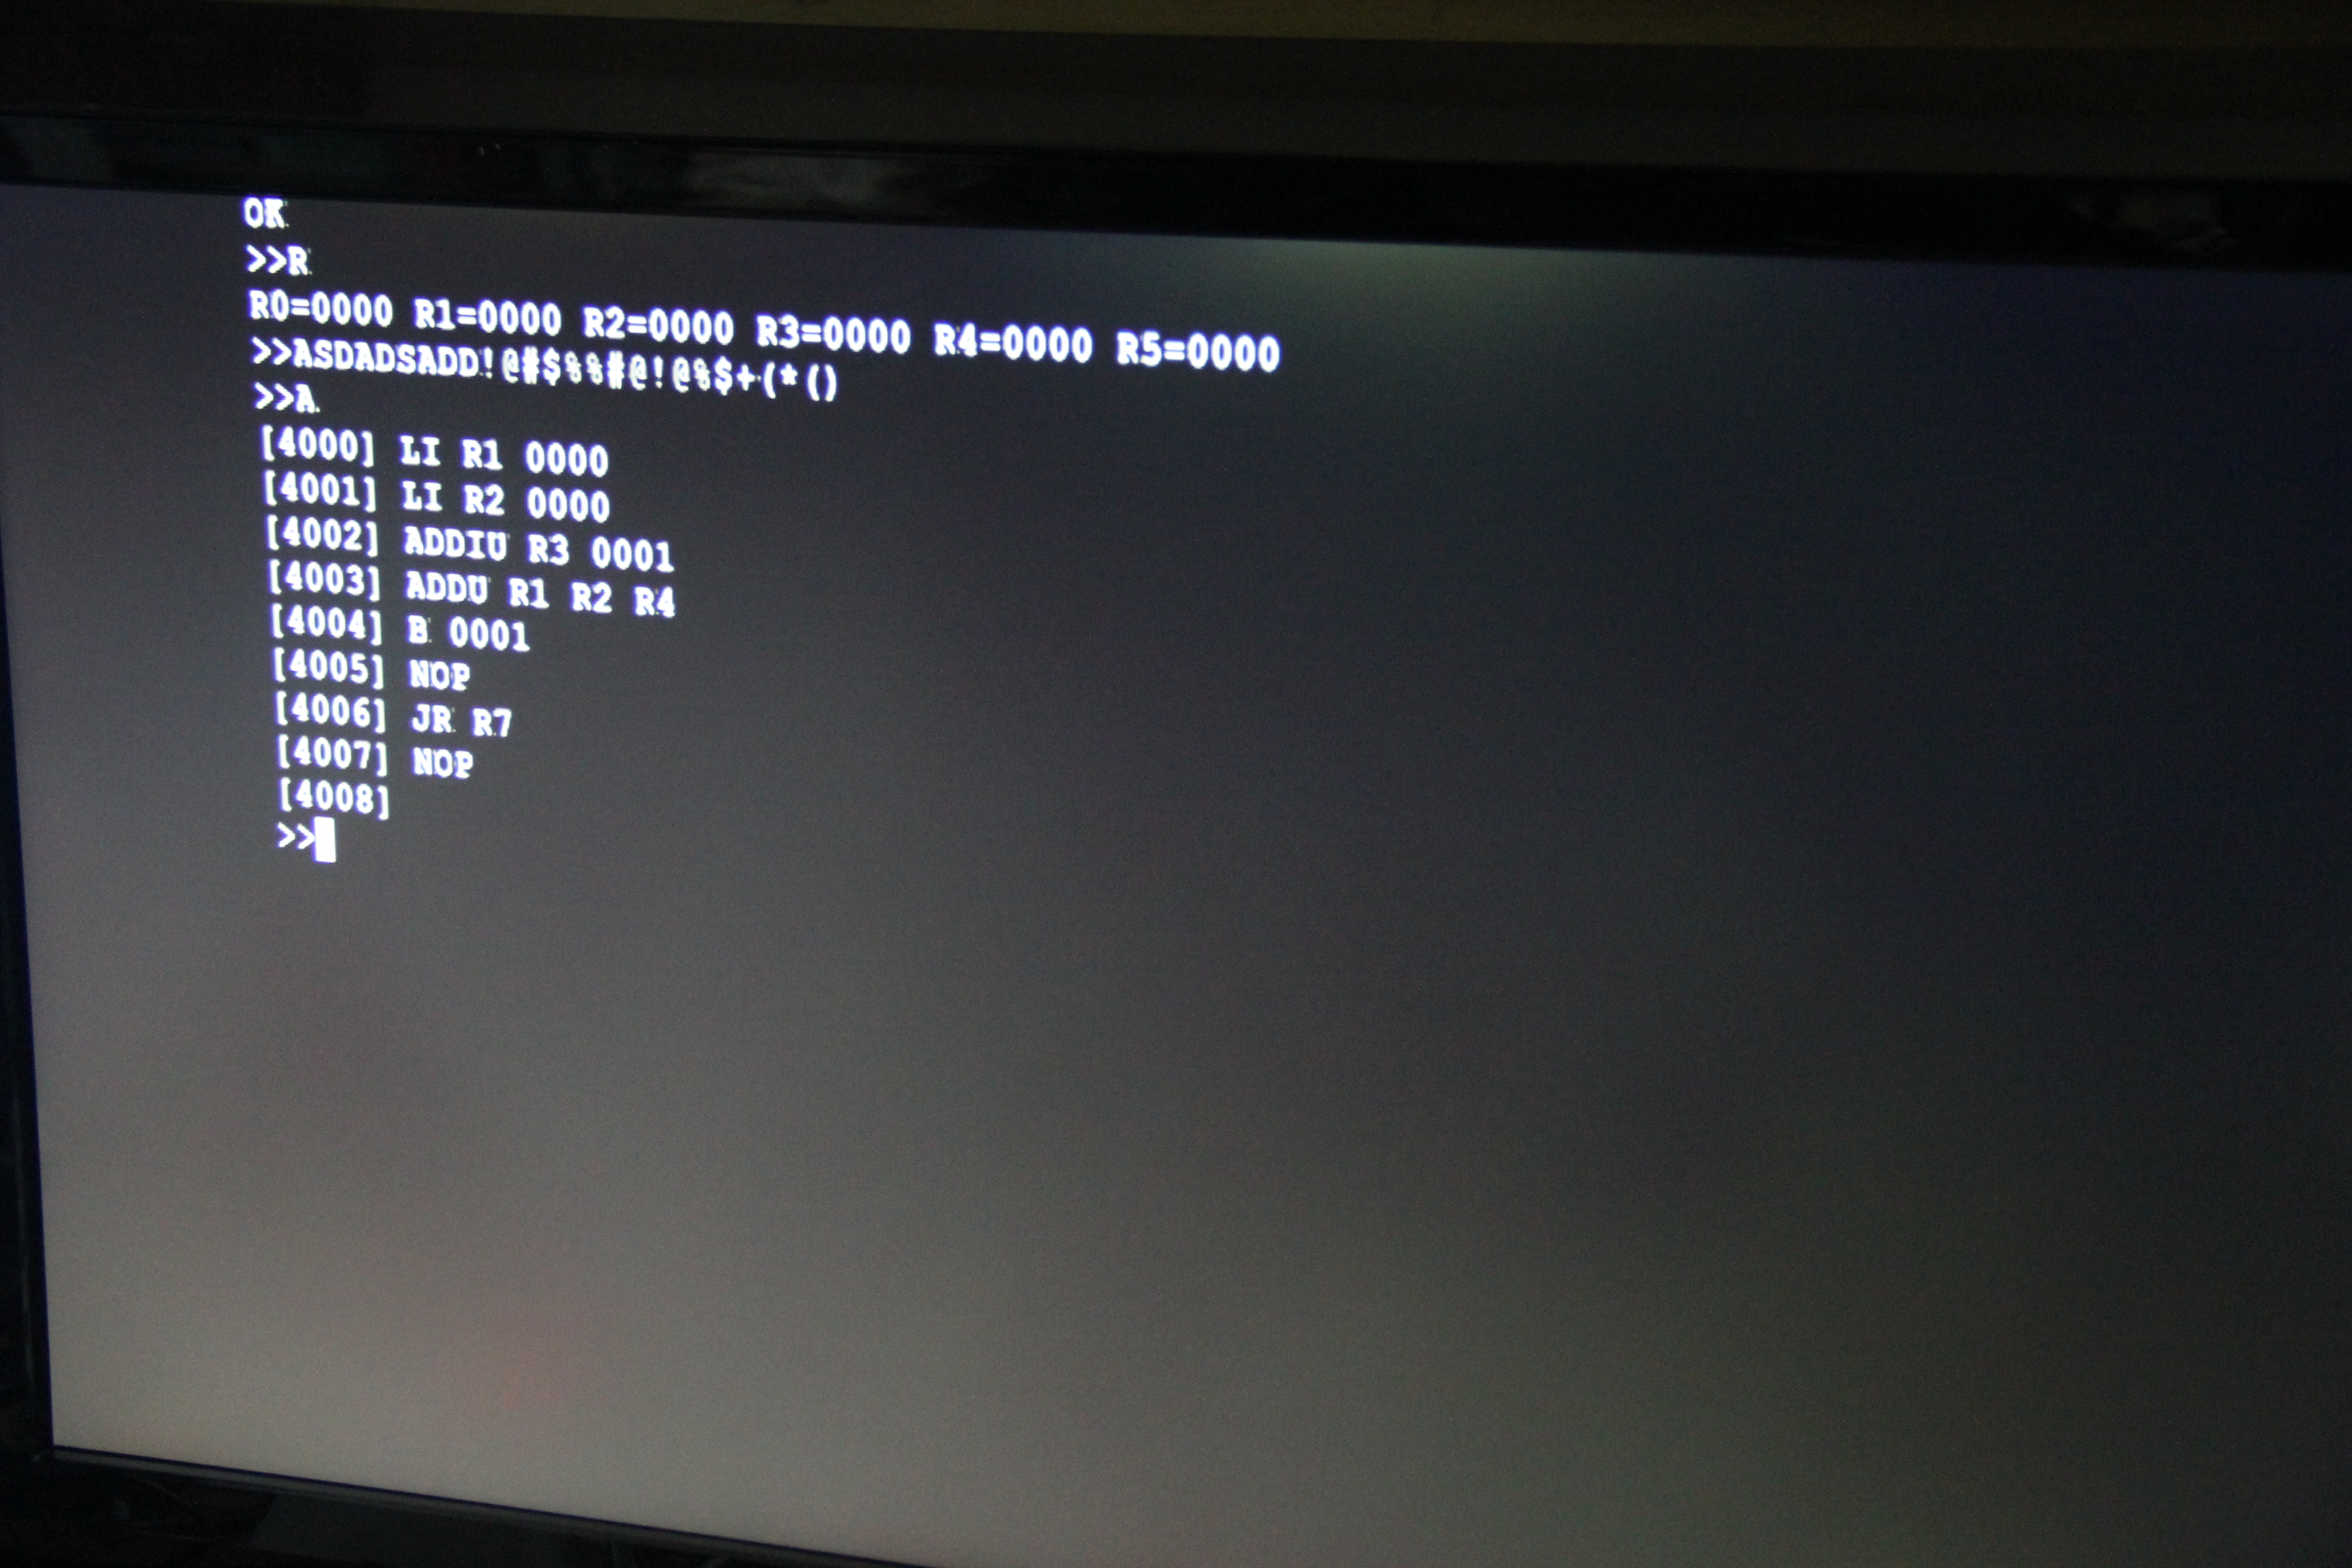
\includegraphics[width=4.5in]{Figures/picture/IMG_7235.JPG}
  \caption{A指令}
\end{figure}

\begin{figure}[H]
  \centering
  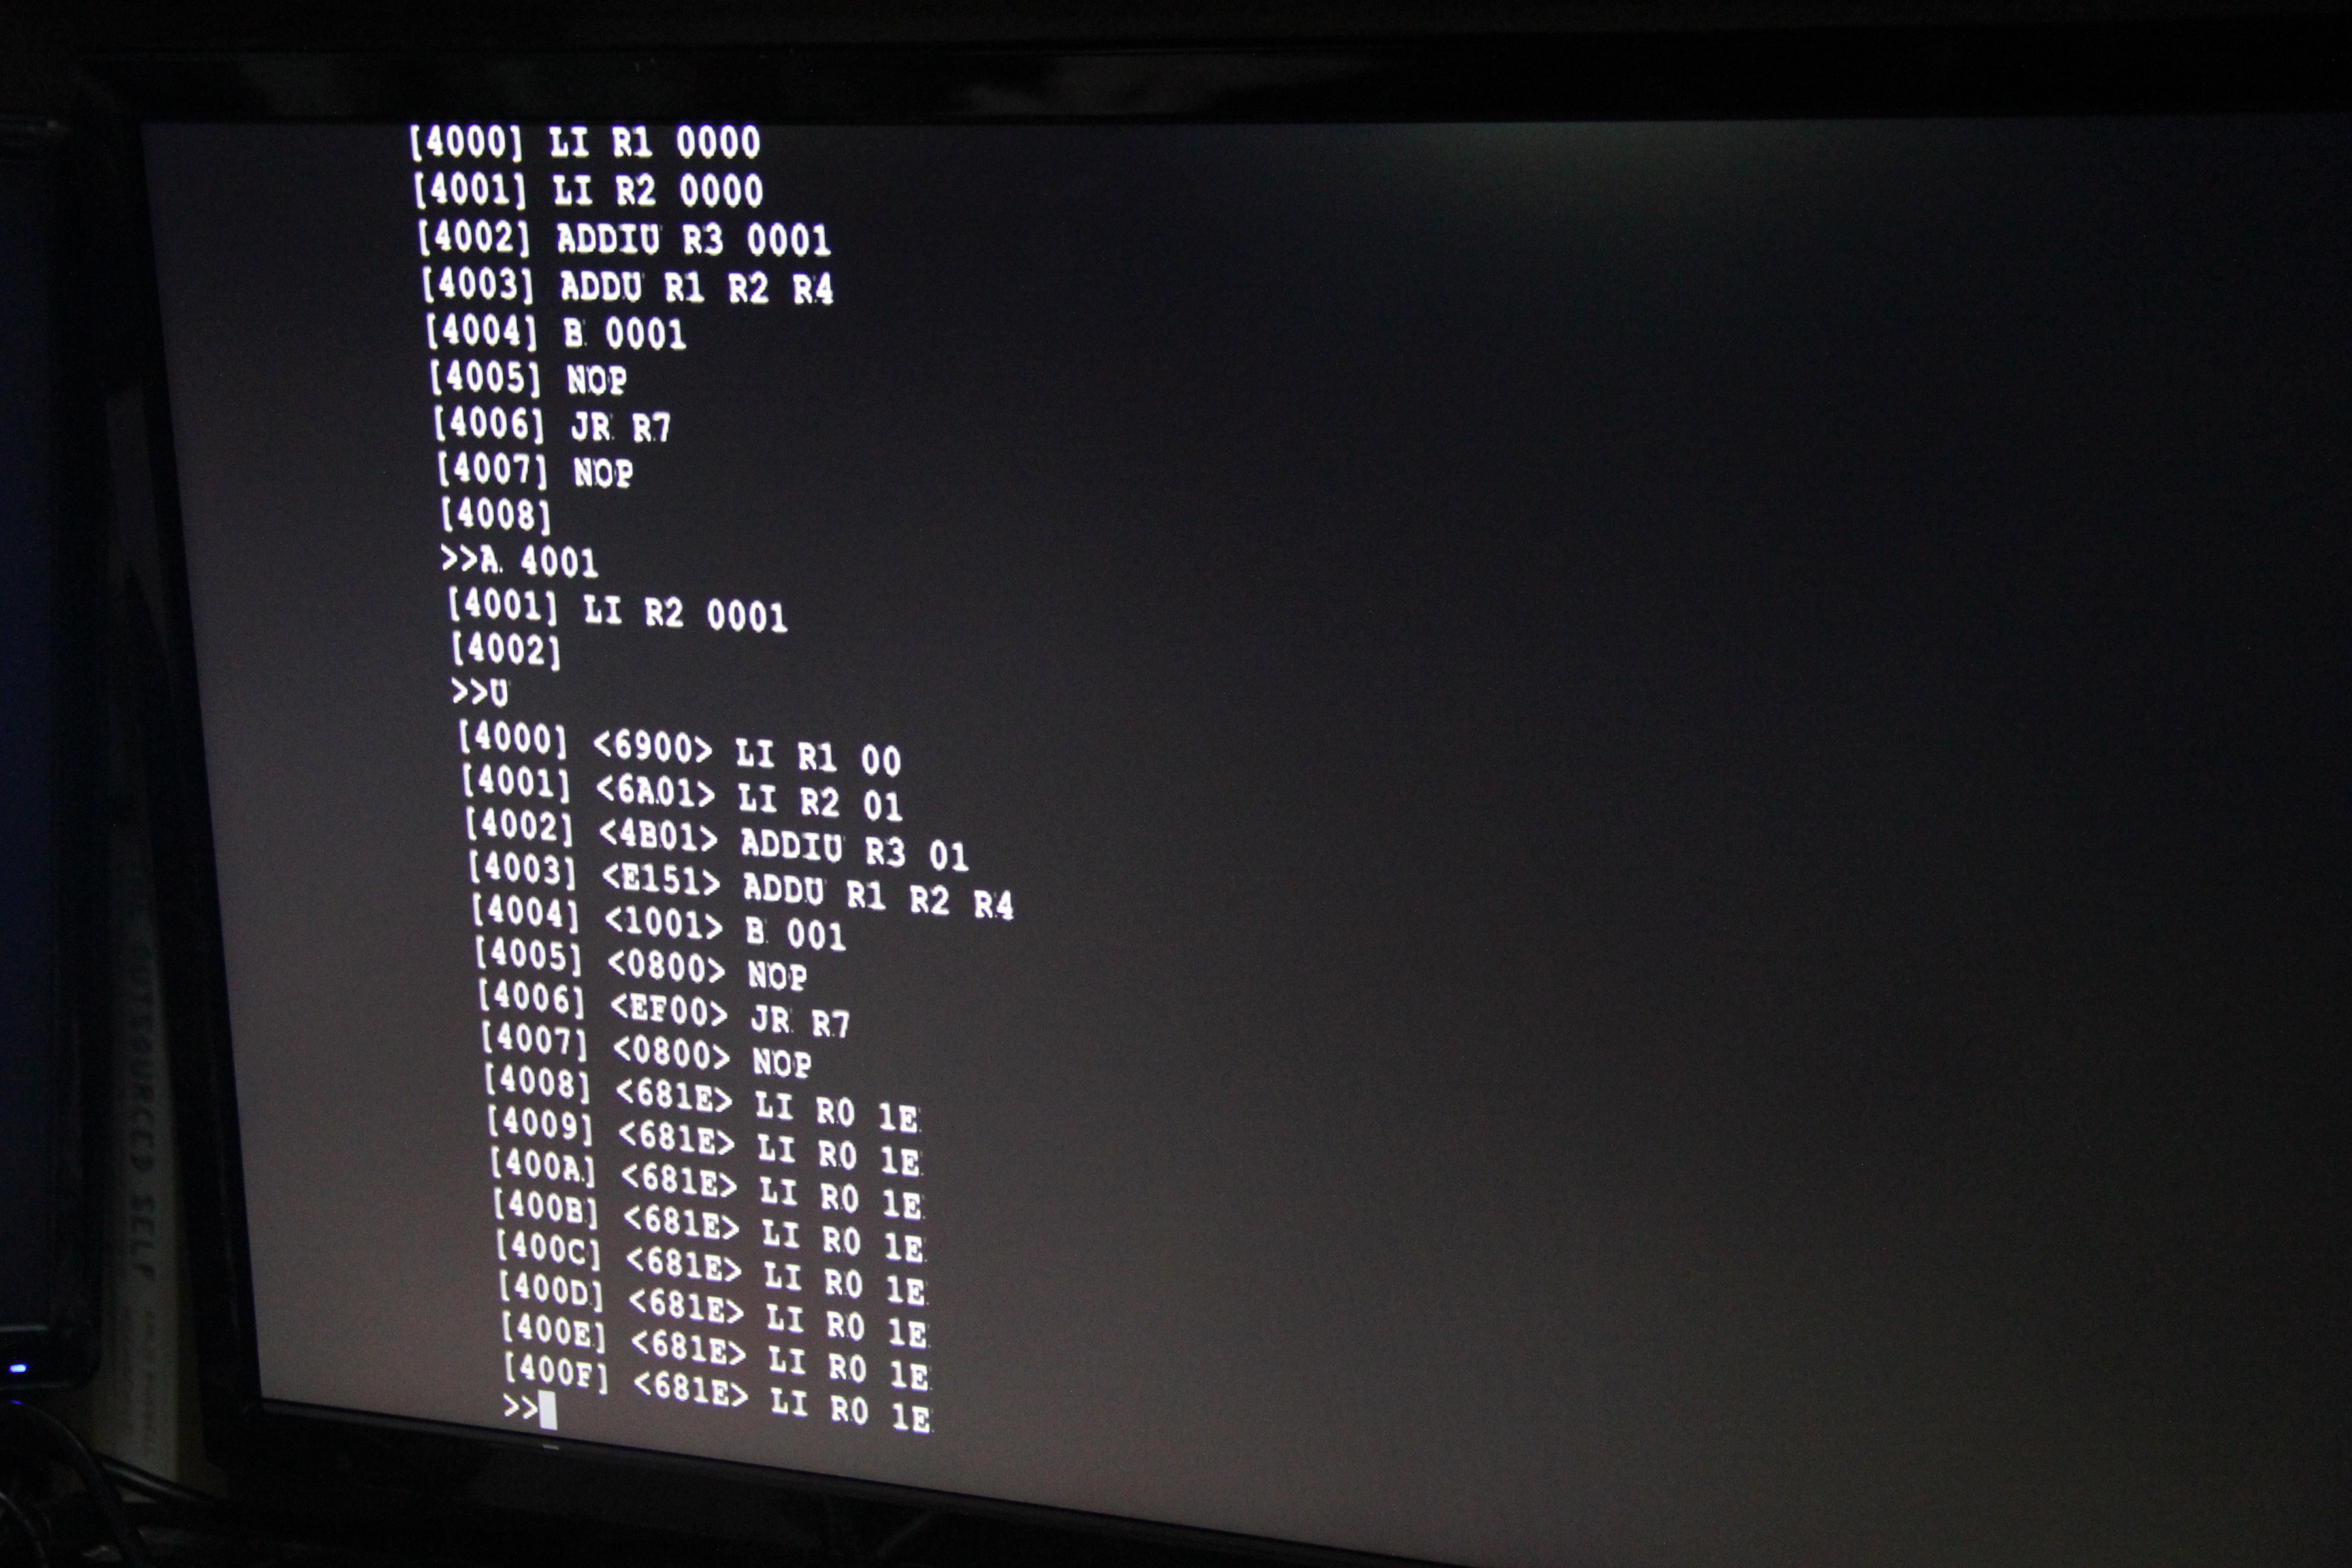
\includegraphics[width=4.5in]{Figures/picture/IMG_7236.JPG}
  \caption{U指令}
\end{figure}

可以看到,指令已经被正确地写入了。此时,我们输入斐波那契数列计算的汇编码,并运行,通过D指令查看内存的值以显示结果是否正确。

\begin{figure}[H]
  \centering
  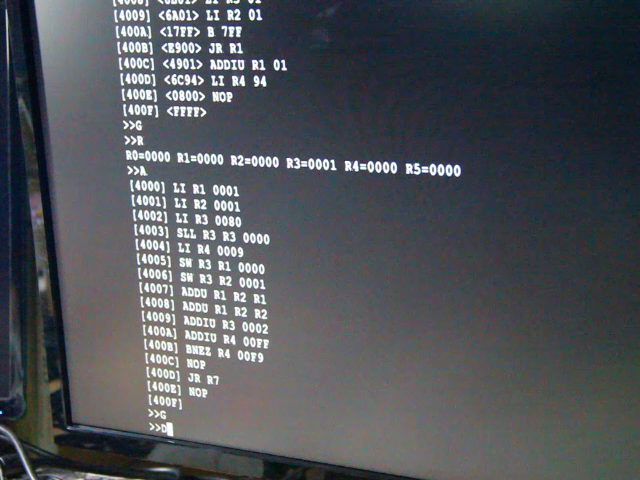
\includegraphics[width=4.5in]{Figures/picture/vlcsnap-2015-12-09-23h47m55s801.png}
  \caption{G指令}
\end{figure}

\begin{figure}[H]
  \centering
  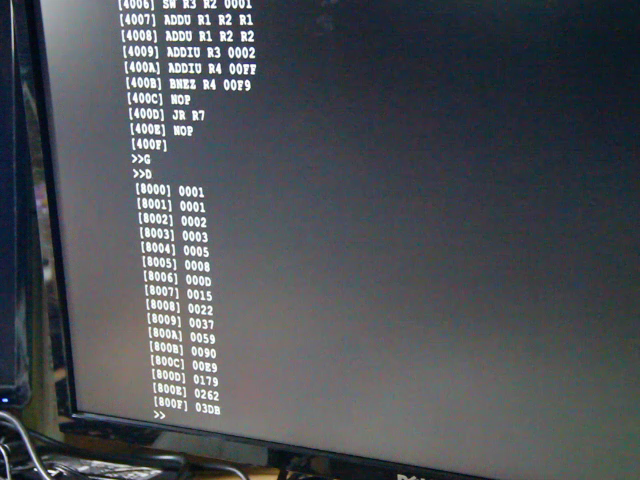
\includegraphics[width=4.5in]{Figures/picture/vlcsnap-2015-12-09-23h48m01s993.png}
  \caption{D指令}
\end{figure}

以上D指令内存的值表示斐波那契数列被正确地计算。最后,我们演示一下Control C中断。通过写入一个死循环程序,G指令运行,通过Ctrl-C组合键退出,并输出中断信息。

\begin{figure}[H]
  \centering
  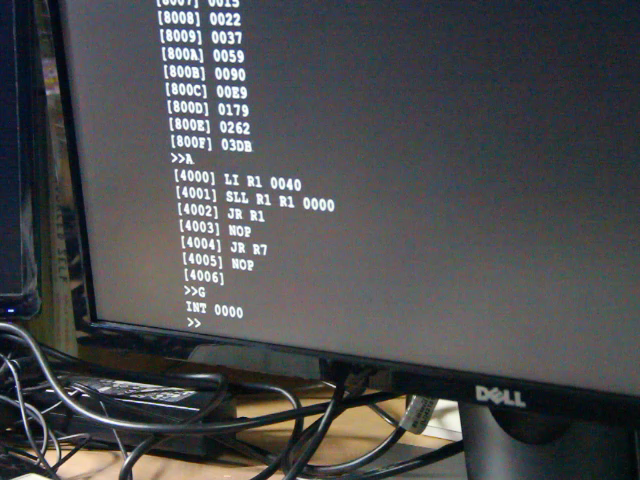
\includegraphics[width=4.5in]{Figures/picture/vlcsnap-2015-12-09-23h48m27s710.png}
  \caption{D指令}
\end{figure}



%----------------------------------------------------------------------------------------
%	SECTION 3
%----------------------------------------------------------------------------------------

\section{多道程序}

在多道程序的CPU,我们同时运行两套监控程序,一个为电脑端term程序,另一个为键盘VGA显示term程序。两套程序均可正确运行。

程序烧入后,可以看到电脑与VGA上均显示出OK。

\begin{figure}[H]
  \centering
  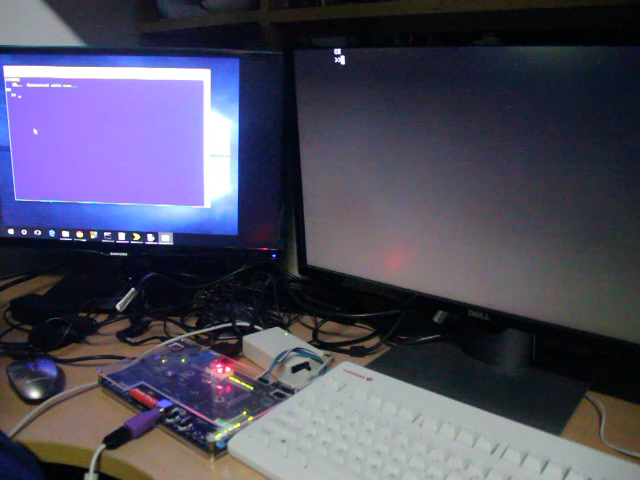
\includegraphics[width=4.5in]{Figures/picture/vlcsnap-2015-12-10-00h17m16s488.png}
  \caption{多道程序初始化}
\end{figure}

我们在电脑term终端输入几条指令到0x4000地址,并通过键盘VGA版的U指令查看写入的指令是否正确。

\begin{figure}[H]
  \centering
  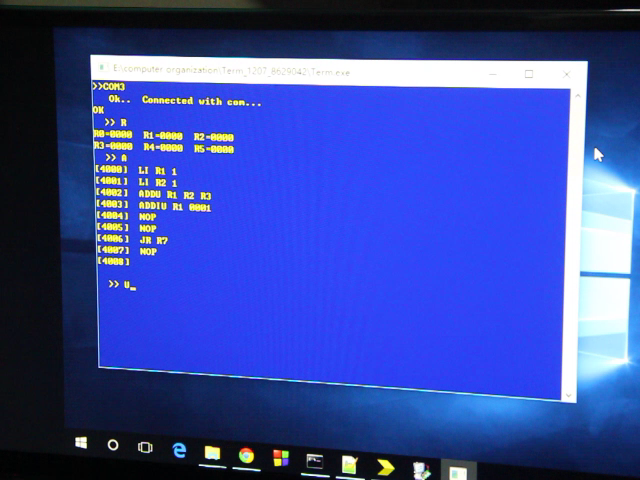
\includegraphics[width=4.5in]{Figures/picture/vlcsnap-2015-12-10-00h17m47s086.png}
  \caption{电脑端A、U指令}
\end{figure}

\begin{figure}[H]
  \centering
  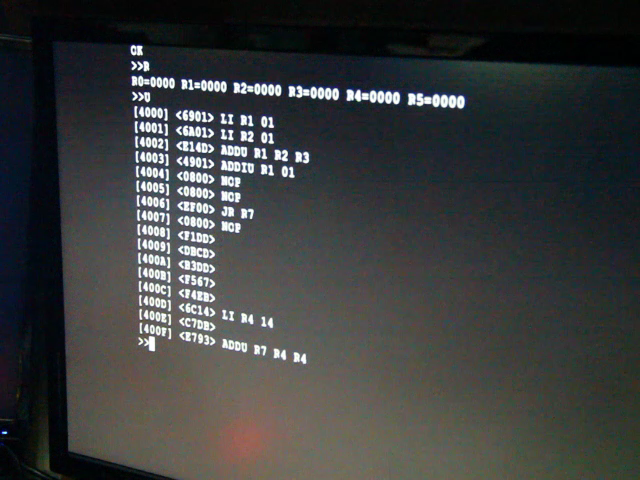
\includegraphics[width=4.5in]{Figures/picture/vlcsnap-2015-12-10-00h18m07s281.png}
  \caption{VGA端U指令}
\end{figure}

在键盘VGA版term程序中通过A指令更改某一条指令,并通过电脑端term查看更改是否正确。

\begin{figure}[H]
  \centering
  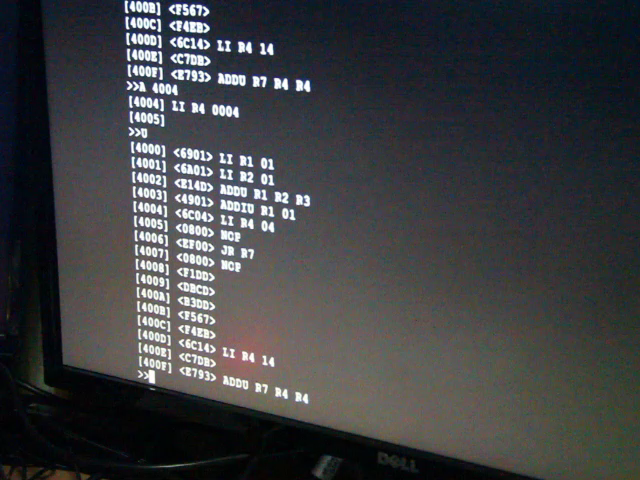
\includegraphics[width=4.5in]{Figures/picture/vlcsnap-2015-12-10-00h18m33s048.png}
  \caption{VGA端A、U指令}
\end{figure}

\begin{figure}[H]
  \centering
  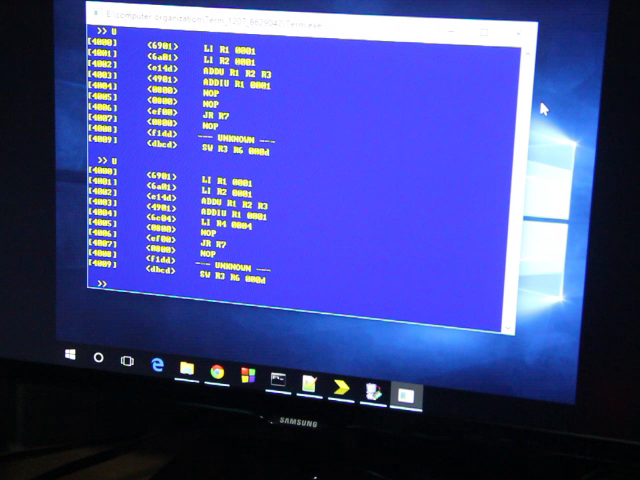
\includegraphics[width=4.5in]{Figures/picture/vlcsnap-2015-12-10-00h18m41s120.png}
  \caption{电脑端U指令}
\end{figure}

电脑端term运行指令,通过R查看寄存器的值是否改变。

\begin{figure}[H]
  \centering
  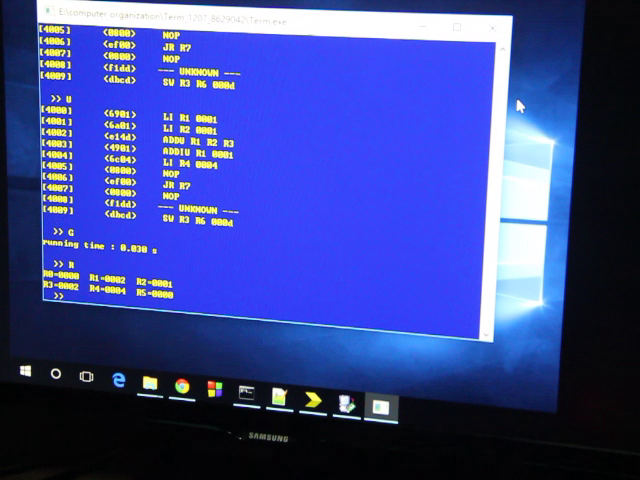
\includegraphics[width=4.5in]{Figures/picture/vlcsnap-2015-12-10-00h19m17s659.png}
  \caption{电脑端R指令}
\end{figure}

在VGA终端查看寄存器的值,发现没有改变,说明两套监控程序的寄存器相互独立。然后运行之前的指令,再次查看寄存器值,发现变为了与电脑端一样。

\begin{figure}[H]
  \centering
  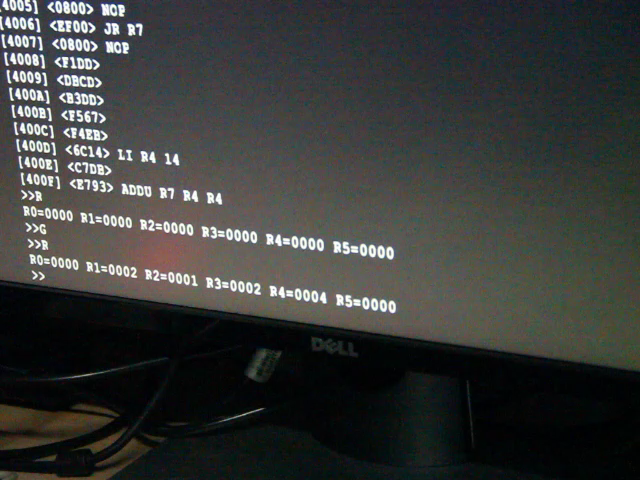
\includegraphics[width=4.5in]{Figures/picture/vlcsnap-2015-12-10-00h19m57s104.png}
  \caption{VGA端R指令}
\end{figure}

以上的演示说明了我们多道程序的正常工作,同时两套监控程序完全独立,也展示出了我们编写CPU作业的亮点。


